\chapter{Hired Guns}

This lecture resumes the argument exactly where the previous one stopped. If government rests on consent, what are the limits on what even a majority may rightly authorize? Sandel sharpens that question by moving from property to life, then from political authority to military recruitment, and finally from military service to reproduction and surrogacy. The argument unfolds in pairs: taxation and conscription, draft and market, coercion and commodification, use and higher modes of valuation. By the end of the lecture we have not solved the problem of consent, but we have learned how to ask it more carefully.

\section{From Taxation to Conscription}

Sandel begins with Locke's view of taxation. A democratically elected government may tax for the common good, and this does not require the present consent of each individual at the moment the tax is enacted or collected. What matters is the prior act of joining political society and accepting the authority of majority rule.

\begin{equation}
\text{prior consent to join political society} \Longrightarrow \text{being bound by majority rule}
\end{equation}

This is the point from which the lecture departs. Once taxation is granted, the harder case comes into focus. If the state may take property without fresh individual consent, may it also conscript citizens and command them to risk their lives? That question seems to press directly against the idea that we own ourselves.

\begin{equation}
\text{taxation without fresh individual consent} \not\Rightarrow \text{conscription is illegitimate}
\end{equation}

So the inquiry changes register. We are no longer asking only what government may tax. We are asking whether consent can ground an obligation that reaches as far as military service and the risk of death.

\section{Arbitrary Power and the Lockean Limit}

Locke's answer, as Sandel presents it, is surprisingly strong. Yes, government may conscript, provided its authority is not arbitrary. The decisive distinction is not between command and non-command, but between rightful law and corrupt will.

\begin{equation}
\text{legitimate authority} \Longrightarrow \text{non-arbitrary rule of law}
\end{equation}

Sandel's favored illustration is Locke's example of the sergeant and the soldier. A sergeant may order a soldier toward the cannon, where death is nearly certain. A general may punish desertion with death. Yet neither officer may arbitrarily take a penny from the soldier's purse. Power over life and death can belong to military office; arbitrary seizure cannot.

\begin{align}
\text{command a soldier into danger} &\text{ may be legitimate},\\
\text{take a penny arbitrarily} &\text{ is corrupt.}
\end{align}

The point is not that consent dissolves all limits. The point is that consent creates political obligation in a form already structured by the rule of law. Government remains limited, but it is limited chiefly by the requirement that it govern through general, non-arbitrary law.

\subsection{Question \& Answer}

\paragraph{Question.} If we own ourselves, how can government ever command us to fight?

\paragraph{Answer.} Sandel's Lockean answer is that the morally decisive consent is not consent to each tax or each military order taken one by one. It is the prior consent to enter political society and to be bound by lawful authority. Self-possession therefore does not by itself exclude conscription. What excludes a command is arbitrariness, not merely its seriousness.

Sandel closes this opening movement by asking why consent should be such a powerful moral instrument in the first place. Rather than answer abstractly, he turns to a concrete case: military recruitment in wartime.

\section{Recruitment Options and the Civil War Hybrid}

The contemporary setting is the Iraq war. Suppose the United States cannot meet its recruitment targets. What should it do? Sandel lays out three possible responses. The accepted classroom slide shows the first two; the transcript immediately adds the third.

\begin{figure}[h]
\centering

\includegraphics[width=0.82\textwidth]{lecture_05_figure_02.png}
\caption{Recruitment options: higher pay or a draft. The third option, outsourcing, is supplied by the spoken continuation rather than the slide itself.}
\end{figure}

The slide itself displays only the first two items:
\begin{enumerate}
\item Increase pay and benefits.
\item Shift to military conscription (a draft).
\end{enumerate}

The transcript then completes the decision set by adding outsourcing to mercenaries. In note form we can write the full menu as

\begin{equation}
\text{recruitment shortfall} \Longrightarrow
\begin{cases}
\text{increase pay and benefits},\\
\text{conscription by lottery},\\
\text{outsource to mercenaries}.
\end{cases}
\end{equation}

Sandel immediately polls the room. A large majority favor higher pay, only a handful favor conscription, and a noticeable minority are drawn to outsourcing. This matters because the lecture is not content to classify opinions. It asks what principle would justify any of these choices.

To sharpen the issue, Sandel inserts an intermediate case from American history: the Civil War draft with a buyout provision. One begins with conscription, but a draftee may hire a substitute to fight in his place. The market enters not at the edge but inside the draft itself.

\begin{equation}
\text{conscription}
\to
\text{Civil War buyout}
\to
\text{all-volunteer army}
\to
\text{outsourcing}
\end{equation}

This progression is a reconstruction of the lecture's logic. It shows the pressure of the argument: once we allow money to reallocate military risk, how far should that principle be permitted to run?

\begin{figure}[h]
\centering
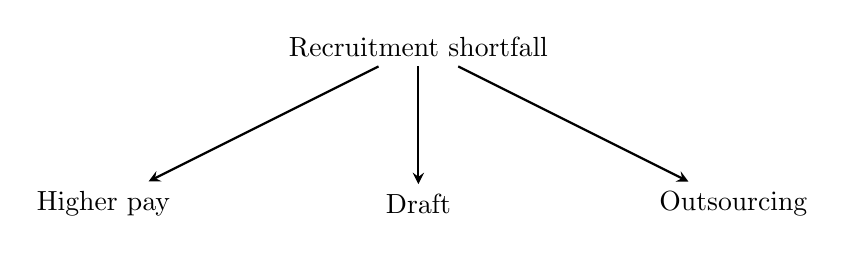
\begin{tikzpicture}[>=stealth, thick]
\node (root) at (0,0) {Recruitment shortfall};
\node (pay) at (-4,-2) {Higher pay};
\node (draft) at (0,-2) {Draft};
\node (out) at (4,-2) {Outsourcing};
\draw[->] (root) -- (pay);
\draw[->] (root) -- (draft);
\draw[->] (root) -- (out);
\end{tikzpicture}
\caption{Transcript-backed reconstruction of the lecture's recruitment decision tree.}
\end{figure}

The Civil War system is the perfect stress test because it is both coercive and marketized. It lets Sandel ask not only who serves, but what kind of good military service is.

\section{Coercion, Inequality, and the All-Volunteer Army}

The first objection surfaces gradually. Liz says the buyout provision puts a price on human life. Jason responds with the libertarian reply: no one is forced to accept the money; if someone sets his own price for risk, why should that be unjust?

Sandel then draws out the deeper criticism from Sam and Raul. The issue is not merely that money changes hands. The issue is that unequal background conditions can make the apparently voluntary exchange only partly free.

As a note-native shorthand, we can express the structure this way:
\begin{equation}
\text{free consent} = \text{voluntariness} + \text{adequate information}
\end{equation}

What Sam and Raul emphasize is the first term. Under conditions of severe inequality, the poor laborer who accepts money to serve in another man's place may be ``choosing,'' but he is choosing under pressure created by circumstance rather than by law alone.

\begin{equation}
\text{severe background inequality} \Longrightarrow
\text{apparently voluntary exchange may be partly coercive}
\end{equation}

Sandel's example makes the asymmetry vivid. For Carnegie the price of substitution is trivial; for a poor laborer the same payment can be decisive. The same market price has different moral significance because it lands within different social situations.

\paragraph{Worked example.} The objection can be written as a short derivation:
\begin{align}
\text{equal draft liability}
&\Longrightarrow \text{buyout option},\\
&\Longrightarrow \text{military burden reallocated by wealth},\\
&\Longrightarrow \text{the poor sell risk under economic pressure},\\
&\Longrightarrow \text{the resulting consent is only partly free.}
\end{align}

Emily then performs the decisive move of the first half of the lecture. Even if we grant the coercion objection in the Civil War case, why does it not also trouble us about the all-volunteer army? Military recruitment today, too, falls disproportionately on those with fewer economic opportunities. Sandel reinforces her point by asking for a quick show of hands about military service in the students' own generation. The result supports the claim that service is not socially distributed at random.

\subsection{Question \& Answer}

\paragraph{Question.} When does a voluntary exchange stop being fully free because inequality is doing the work?

\paragraph{Answer.} The lecture does not give a numerical threshold. It gives a structural test. A voluntary exchange ceases to be fully free when the background distribution of opportunity is so unequal that one side enters the bargain because its alternatives are unacceptably narrow. The form of consent remains, but the substance is compromised.

This is already a powerful argument, but Sandel does not stop there. He allows the discussion to shift from coercion to a different question altogether.

\section{Patriotism, Civic Obligation, and Market Allocation}

Once Emily extends the inequality objection to the all-volunteer army, another line of criticism emerges. Perhaps the problem with paying for military service is not only that it exploits inequality. Perhaps military service is the wrong kind of good to allocate by market exchange.

Jackie argues that patriotism is a better motive than money. Philip replies that mercenaries can fight effectively even without patriotic attachment. Sandel's intervention clarifies what is really at issue. The term ``all-volunteer army'' is, he notes, a kind of misnomer. In practice it is a paid army. So if patriotism should be primary, are we defending the current system, or does that thought push us back toward conscription?

The lecture now separates two objections that had been intermixed in the classroom exchange:

\begin{equation}
\text{objection}_1=\text{coercion under inequality},
\qquad
\text{objection}_2=\text{civic obligation / patriotism}
\end{equation}

The first objection says that the market may fail to secure genuinely free exchange. The second says that military service may be bound up with citizenship in a way that makes market allocation unfitting even if the exchange were fully voluntary.

Sandel also shows how these lines of thought pull in opposite directions. If we follow the logic of market choice consistently, the path runs from conscription to buyout to a paid army and perhaps onward to outsourcing. If, however, patriotism and civic obligation really count for something, then perhaps the market has already gone too far.

At that point Sandel steps back and names the two philosophical questions that the debate has produced:

\begin{equation}
\text{Question 1: what inequalities undermine free labor exchange?}
\end{equation}

\begin{equation}
\text{Question 2: what are the obligations of citizenship?}
\end{equation}

He does not answer either question here. He deliberately leaves them open and carries them into the next domain.

\section{From Military Service to Markets in Reproduction}

The bridge to the second half is perfectly characteristic. Sandel asks whether one should be able to bid for a baby that is up for adoption. The point is not to start a new lecture. The point is to transport the same logic of consent, exchange, and valuation into a domain where our moral intuitions are even less at ease.

He first considers markets in eggs and sperm. A newspaper advertisement seeks not merely any egg donor but one with specified traits and offers an enormous financial inducement, on the order of \$50{,}000, for the right donor. On the sperm side, California Cryobank pays donors per specimen, up to a monthly ceiling, while openly recruiting the traits its customers prefer. The transcript's numerical details are secondary to the structure: reproductive capacities are being priced, screened, and marketed.

Sandel's phrasing is pointed. This is a market in reproductive capacities. And once that is said, the question is no longer merely legal or medical. Should eggs and sperm be bought and sold for money at all? Before the class can settle that question, Sandel introduces the more difficult case of commercial surrogacy, where contract, pregnancy, attachment, and money all converge.

\section{Surrogacy, Contract, and the Limits of Market Reason}

The Baby M case begins in contractual form. The Sterns want a child. Mary Beth Whitehead agrees to be artificially inseminated with William Stern's sperm, to carry the child, and then to surrender the baby for a fee plus expenses.

\begin{equation}
\text{payment} + \text{artificial insemination} + \text{birth} \Longrightarrow \text{transfer of child to the Sterns}
\end{equation}

The first argument Sandel elicits is the contractarian one. Patrick says, in effect, that a deal is a deal. If competent adults knew the terms and agreed voluntarily, the contract should be enforced. Sandel lets that position stand clearly before turning to the objections.

Evan introduces the first objection. Even if the agreement was voluntary, it may not have been informed. Before the child exists, the mother cannot know how she will feel about the child she bears. That means the relevant information was unavailable at the moment of agreement.

\begin{equation}
\text{consent can fail through coercion}
\qquad \text{or} \qquad
\text{consent can fail through inadequate information}
\end{equation}

\begin{equation}
\text{pre-birth consent} \not\Rightarrow \text{fully informed consent}
\end{equation}

Anna adds a stronger appeal to the natural bond between mother and child. Kathleen replies by restoring the strict contractual frame: later feelings do not undo a bargain. Then Andrew introduces the second objection, and with it the lecture's deeper unease. The issue, he says, is not only information. It is that surrogacy begins to look like baby-selling, or at least like the sale of a mother's right to her child.

\subsection{Question \& Answer}

\paragraph{Question.} Can a surrogacy contract be fully voluntary if the mother cannot yet know the bond she will form with the child?

\paragraph{Answer.} Sandel's answer is that voluntariness and informedness must be distinguished. A contract can be entered without overt coercion and still fail to count as fully free if the relevant knowledge is unavailable at the moment of agreement. In the surrogacy case, the court's concern is precisely that the mother is asked to commit herself irrevocably before she can know the force of the attachment pregnancy may create.

Vivian's comparison between sperm donation and surrogacy deepens that point. The biological bond and the temporal labor of pregnancy, she argues, cannot be assimilated to sperm donation. The goods are not equal because the forms of human involvement are not equal.

Sandel then moves from classroom exchange to legal reasoning. The lower court treated the contract as enforceable: a bargain was struck, neither party had a superior bargaining position, and no one forced the other. The New Jersey Supreme Court, however, refused to enforce it. The stable structure of the court's reasoning follows the two objections already heard in the room: insufficiently informed consent and commodification.

\begin{figure}[h]
\centering

\includegraphics[width=0.82\textwidth]{lecture_05_figure_03.png}
\caption{Quote framing the commodification objection to surrogacy.}
\end{figure}

The slide preserves the moral temperature of the second objection. Rather than reproduce the full quotation in the text, we can extract its argumentative core:

\begin{equation}
\text{profit motive predominates and ultimately governs the transaction}
\end{equation}

That lets us summarize the court's two-part structure cleanly:

\begin{equation}
\text{objection}_1=\text{tainted consent},
\qquad
\text{objection}_2=\text{commodification / dehumanization}
\end{equation}

\begin{figure}[h]
\centering
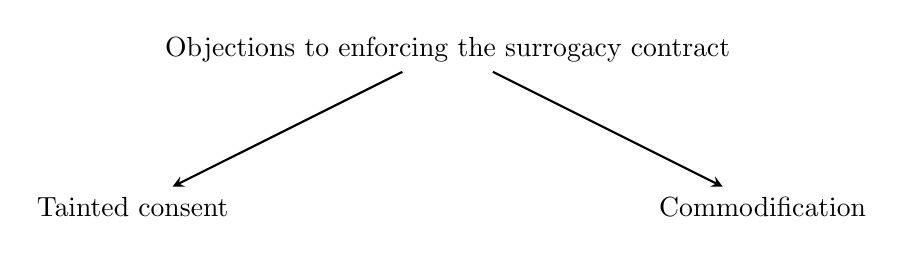
\begin{tikzpicture}[>=stealth, thick]
\node (root) at (0,0) {Objections to enforcing the surrogacy contract};
\node (consent) at (-4,-2) {Tainted consent};
\node (commod) at (4,-2) {Commodification};
\draw[->] (root) -- (consent);
\draw[->] (root) -- (commod);
\end{tikzpicture}
\caption{A note-native reconstruction of the lecture's two-part analysis.}
\end{figure}

The second objection is harder to state precisely, and Sandel says so. Its claim is not simply that one side lacked information. It is that some goods are degraded when they are treated as items for use and profit. To clarify that thought, he turns to Elizabeth Anderson. Her proposal is that surrogacy contracts can transform pregnancy into alienated labor by requiring the mother to divert or repress the very attachment pregnancy ordinarily fosters.

\begin{equation}
\text{surrogacy contract} \Longrightarrow \text{alienated labor}
\end{equation}

From there the lecture opens outward. The problem is no longer only surrogacy. It is whether some goods are properly valued in modes other than use and price.

\begin{equation}
\text{some goods are not properly valued merely by use or price}
\end{equation}

Anderson's vocabulary gives Sandel a compact way to name those alternative modes of valuation:

\begin{equation}
V_{\text{non-market}}
=
\{\text{respect},\ \text{appreciation},\ \text{love},\ \text{honor},\ \text{awe},\ \text{sanctity}\}
\end{equation}

The closing example of Cecil Jacobson reinforces the same distinction. One can condemn him for failing to inform the women he treated; that is the consent objection. But Ellen Goodman's line that fatherhood should be something one does, not something one donates, points toward the deeper question: are there goods whose meaning is damaged when they are translated into market terms? That question carries the lecture to its endpoint.

\section{Summary}

The lecture begins by testing Locke at his strongest point. If prior consent can authorize taxation, can it also authorize conscription? Locke's answer is yes, so long as political and military power are not arbitrary. Sandel then turns that abstract answer into a concrete argument about recruitment, where the market enters and complicates consent. From the Civil War buyout system to the paid army and outsourcing, we are forced to distinguish between exchange that is formally voluntary and exchange that is genuinely free.

The second half repeats the same structure in a more intimate setting. In surrogacy, consent may be flawed not because of overt coercion but because crucial information is unavailable before birth. And beyond the problem of consent lies the harder issue of commodification: whether some human goods are not properly valued as objects of purchase. The lecture therefore leaves us with two persistent questions. When is consent morally sufficient? And what kinds of goods are corrupted when market reasoning becomes their governing logic? Sandel does not close those questions here. He leaves them alive for the lectures to come.